\section{Introduction}
A client dominated by one class must use a shared model that also serves nineteen other label distributions. In our label-skewed CIFAR-10 setting, the shared model reaches 38.96\% client-macro accuracy, below the 63.06\% obtained by predicting from local class frequencies alone. Figure~\ref{fig:motivation} motivates interpreting shared logits locally~\cite{mcmahan2017fedavg,arivazhagan2019fedper,chen2022fedrod}.

Fixed unit-strength prior addition uses a preset offset; vector scaling supplies no client-prior center~\cite{menon2021logitadjust,guo2017calibration}. Fixed addition can duplicate information in shared logits; an unconstrained fit must infer it from limited local labels.

We shrink the bias toward the client's prior instead of adding it. Infinite regularization fixes the prior offset; vanishing regularization removes the penalty. At an optimum, $\lambda(b-\mu)=n-\sum p$: bias deviations track observed counts minus fitted probability mass; agreeing centers are retained and disagreeing ones corrected.

Personalization decides what each client predicts; it does not decide what each client sends. Compressed bytes alone identify neither their client--round context nor the model state that incorporated them. Lost responses, duplicate delivery and replay can separate upload history from the residual used in the next round. We bind each encoded update to its round context and advance the residual through an authenticated incorporation receipt. We call the resulting system prior-regularized lightweight federated learning (PR-LFL).

\begin{figure}[!htb]\centering
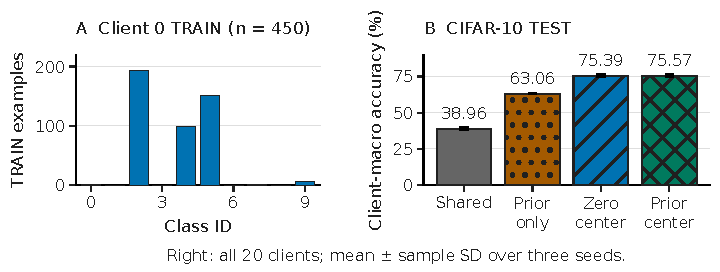
\includegraphics[width=0.9\linewidth]{figures/motivation_route_a.pdf}
\caption{Local counts expose the prediction gap. Left: CIFAR client 0 TRAIN. Right: client-macro accuracy over twenty clients and three seeds, including prior-only prediction.}\label{fig:motivation}
\end{figure}

\paragraph{Contributions.}
(i) A twenty-parameter prior-centered predictor addresses label heterogeneity, lowering NLL across all three fixed seeds on both tasks; in this three-point sweep, mean gain increases as heterogeneity strengthens. (ii) Ledger anchoring binds compressed payloads to their round context, and an authenticated incorporation receipt gates error-feedback residual commitment. (iii) Measurements establish 54,067 B codec uploads and 4.23 M gas for fifteen registrations across five clients and three rounds; four fault classes recover the recorded contribution and residual transition.

\section{Related Work}
\paragraph{Personalization.}
FedProx, SCAFFOLD and FedNova change shared optimization~\cite{li2020fedprox,karimireddy2020scaffold,wang2020fednova}. FedPer/FedRoD retain personal heads; Ditto/pFedMe regularize personal models; FedBN retains local normalization~\cite{li2021ditto,dinh2020pfedme,li2021fedbn}. Quantization, sparsification and error feedback reduce traffic~\cite{alistarh2017qsgd,stich2018sparsified,karimireddy2019errorfeedback}. PR-LFL combines local prediction with a state-preserving compressed-upload path.

\paragraph{Class priors and calibration.}
Prior estimation, logit adjustment, Balanced Softmax and FedLC use class counts in prediction or training~\cite{saerens2002prior,lipton2018bbse,menon2021logitadjust,ren2020balanced,zhang2022fedlc}. PRIOR learns Bregman regularization centers~\cite{shi2023prior}; vector scaling, BCTS and Dirichlet calibration transform scores~\cite{guo2017calibration,alexandari2020labelshift,kull2019dirichlet}. LaSCal adapts temperature under label shift~\cite{popordanoska2024lascal}; calibration studies motivate uncertainty metrics~\cite{vaicenavicius2019calibration,kumar2019verified,ovadia2019shift}. FedCal and private federated calibration learn scalers, while FedNPC retrains a server classifier~\cite{peng2024fedcal,maddock2025privatecal,gao2026fednpc}. We center a compact frozen-logit fit on each client's observed log class frequencies.

\paragraph{Ledger-anchored federated learning.}
BlockFL exchanges and verifies local model updates through blockchain coordination~\cite{kim2020blockfl}. Biscotti combines a ledger of model updates with cryptographic commitments and secure aggregation~\cite{shayan2021biscotti}. We bind each record to the learning state through authenticated incorporation and residual commitment, extending the record beyond a stored hash.
